\section{Results}
\label{sec:results}
Unless stated otherwise, we report query-macro percentages on the primary populations, percentage-point (pp) differences, and nDCG on the 0--1 scale.

\subsection{Attribute-Order Sensitivity (RQ1)}
Across the seven catalog-wide schedules, VI@20 ranges from 11.93--19.58\% on WANDS and 3.66--6.91\% on ESCI. These estimates describe crossing within the tested family, not a probability of omission under future orders.

With every competitor fixed at source order, changing only the target yields VI@20 of 10.83--19.45\% on WANDS and 2.42--5.88\% on ESCI. The interventions answer complementary questions; their difference does not decompose target and competitor effects. Sensitivity remains when every tested target input fits completely: fully-fitting VI@20 ranges from 7.16--14.55\% and 2.55--5.88\%, respectively (Figure~\ref{fig:rq1_target_fitting}). GTE's full and fitting populations coincide. MiniLM and BGE fitting subsets differ from the full populations and from one another, so these comparisons do not isolate a causal truncation or architecture effect.

\begin{figure*}[t]
\centering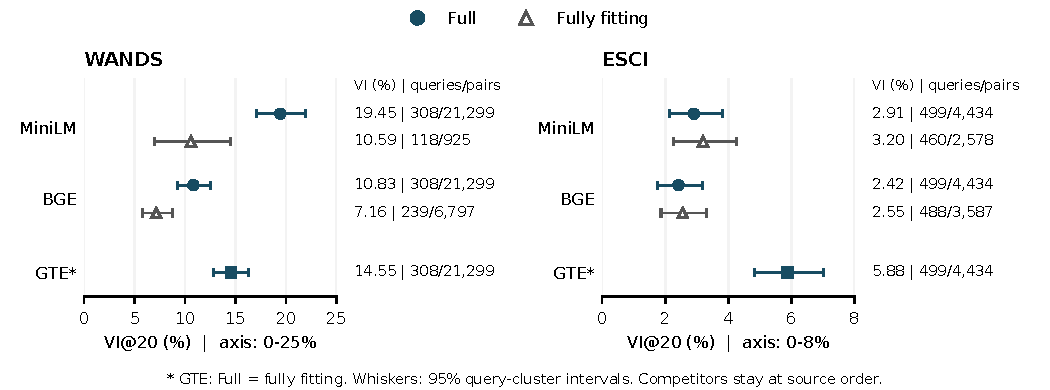
\includegraphics[width=\textwidth]{figures/figure3_target_fitting.pdf}
\caption{Target-only VI@20 with 95\% query-cluster intervals and query/pair support. GTE shows one estimate for identical full and fitting populations. Panel axis ranges differ explicitly; competitors remain fixed.}
\label{fig:rq1_target_fitting}
\Description{Separate markers show full and fitting estimates, without a connecting line implying a truncation intervention.}
\end{figure*}

On the frozen 128-query WANDS supplement, expanding the harmonized family from seven to 32 schedules increases target-only VI@20 by 7.18 pp (95\% CI [5.73, 8.89]) for MiniLM and 6.09 pp (95\% CI [4.56, 7.81]) for BGE, with the full execution comparison and common fitting supports in the supplement.

\subsection{Aggregate Effectiveness and Product Membership (RQ2)}
Gains and losses can be substantially larger than their net Recall change. Reversing WANDS attributes with BGE newly includes 2.357\% and newly omits 2.263\% of highest-label support. The full-precision sum rounds to 4.621\%, while Recall changes by only $+0.094$ pp (95\% CI $[-0.409,0.563]$). Each share is divided by $|H_q|$ within a query before macro averaging.

Exact replacement also occurs within individual queries. For this reversal, 73 of 308 WANDS/BGE queries (23.70\%) have equal positive gain and loss counts. Across the six contrasts, counts range from 67 to 78 (21.75--25.32\% per contrast), not a union of distinct queries. Figure~\ref{fig:rq2_membership} uses reversal as the same definition-based editorial contrast in every setting, selected after historical outcomes; all original schedules remain in companion outputs. In the same catalog-wide reversal, an illustrative hash-selected query, ``anti fatigue mat,'' exchanges five Exact products in each direction while Recall@20 remains exactly $20/307$. The case companion records every changed ID, name, label, rank and order.

\begin{figure*}[t]
\centering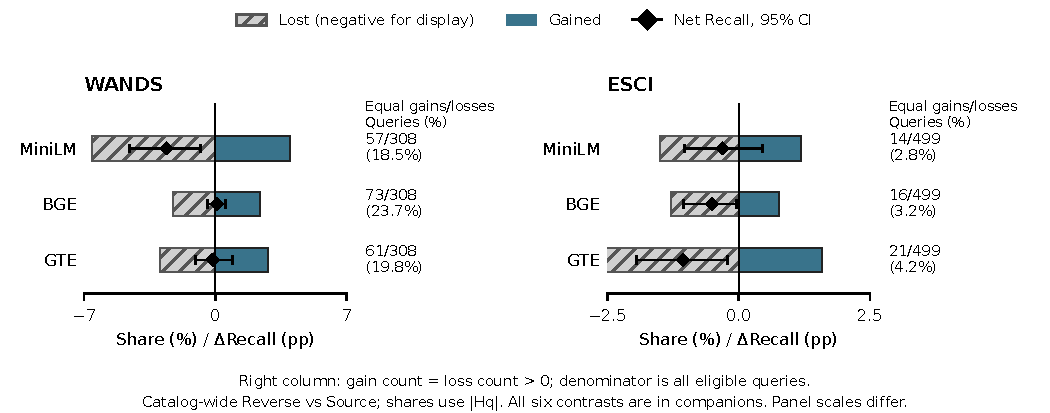
\includegraphics[width=\textwidth]{figures/figure4_membership_replacement.pdf}
\caption{Catalog-wide Reverse versus source at $K=20$. Bars show query-macro gained/lost shares of $H_q$; losses are nonnegative quantities drawn left only for display. Diamonds show net Recall differences with 95\% paired intervals. Counts require equal positive integer gains and losses and use all eligible queries as denominator.}
\label{fig:rq2_membership}
\Description{Relevant membership turnover can exceed net Recall changes, and individual queries can have unchanged Recall with different relevant products.}
\end{figure*}

Graded effectiveness is complementary. Conditional on changed Top-20 relevant membership, median absolute nDCG@20 differences range from 0.0226--0.0399 on WANDS and 0.0388--0.0482 on ESCI. Signed means over all eligible queries range from $-0.01101$ to $+0.00151$ and $-0.00393$ to $+0.00092$, respectively. These summarize different populations and quantities. The companion retains each named contrast, its unadjusted interval, condensed nDCG and judged coverage; intervals containing zero do not establish equality.

\subsection{Effectiveness and Consistent Inclusion under Controls (RQ3)}
Canonical, set-based, fixed-view and lexical controls remove incoming-order dependence by construction. Their zero VI is structural; effectiveness and which products are persistently included remain empirical questions. Table~\ref{tab:strategy_joint} retains all three canonical rules without choosing a test winner. Raw dense and raw hybrid effectiveness average seven schedules; source-order results remain separately labelled in the companion.

\begin{table*}[t]
\centering\normalsize\setlength{\tabcolsep}{6pt}\renewcommand{\arraystretch}{1.05}
\caption{Common-support controls. Recall (R) and VI are percentages; nDCG uses 0--1. R@100/VI@100 assess candidate inclusion, whereas nDCG@20 assesses ranking near the top. All fixed controls have structural VI=0. The companion includes R@20, paired intervals, source-order references, GTE and every view budget.}
\label{tab:strategy_joint}
% Audited candidate. Requires booktabs. Two-column table; R/VI@100 for candidates, nDCG@20 for top ranks.
\begin{tabular}{lrrrrrr}
\toprule
Method & \multicolumn{3}{c}{MiniLM} & \multicolumn{3}{c}{BGE} \\
 & R@100 & VI@100 & nDCG@20 & R@100 & VI@100 & nDCG@20 \\
\midrule
\multicolumn{7}{l}{WANDS} \\
Raw dense (7 mean) & 56.61 & 21.89 & 0.6323 & 63.62 & 12.30 & 0.7008 \\
Canonical: ascending & 56.05 & 0.00 & 0.6264 & 63.24 & 0.00 & 0.6981 \\
Canonical: descending & 56.16 & 0.00 & 0.6341 & 63.61 & 0.00 & 0.7023 \\
Canonical: type priority & 57.19 & 0.00 & 0.6312 & 63.56 & 0.00 & 0.7030 \\
BM25 & 63.23 & 0.00 & 0.6548 & 63.23 & 0.00 & 0.6548 \\
Raw hybrid (7 mean) & 65.55 & 11.08 & 0.6983 & 67.77 & 7.05 & 0.7254 \\
Canonical hybrid: ascending & 65.61 & 0.00 & 0.6960 & 68.15 & 0.00 & 0.7239 \\
Canonical hybrid: descending & 65.29 & 0.00 & 0.6979 & 67.93 & 0.00 & 0.7272 \\
Canonical hybrid: type priority & 65.71 & 0.00 & 0.6988 & 67.83 & 0.00 & 0.7262 \\
Set-Mean & 58.81 & 0.00 & 0.6366 & 61.82 & 0.00 & 0.6841 \\
\midrule
\multicolumn{7}{l}{ESCI} \\
Raw dense (7 mean) & 86.19 & 1.41 & 0.6019 & 91.04 & 0.72 & 0.6623 \\
Canonical: ascending & 86.41 & 0.00 & 0.6015 & 91.05 & 0.00 & 0.6632 \\
Canonical: descending & 86.38 & 0.00 & 0.6008 & 91.01 & 0.00 & 0.6612 \\
Canonical: type priority & 86.36 & 0.00 & 0.6013 & 91.09 & 0.00 & 0.6629 \\
BM25 & 82.83 & 0.00 & 0.6151 & 82.83 & 0.00 & 0.6151 \\
Raw hybrid (7 mean) & 89.57 & 0.56 & 0.6404 & 91.61 & 0.74 & 0.6690 \\
Canonical hybrid: ascending & 89.51 & 0.00 & 0.6392 & 91.55 & 0.00 & 0.6710 \\
Canonical hybrid: descending & 89.66 & 0.00 & 0.6405 & 91.55 & 0.00 & 0.6690 \\
Canonical hybrid: type priority & 89.54 & 0.00 & 0.6392 & 91.57 & 0.00 & 0.6709 \\
Set-Mean & 84.50 & 0.00 & 0.5887 & 88.95 & 0.00 & 0.6371 \\
\bottomrule
\end{tabular}

\end{table*}

Simple controls have setting-dependent effectiveness. Set-Mean's Recall@100 exceeds the raw dense seven-schedule mean on WANDS/MiniLM and is lower in the other three MiniLM/BGE settings. Raw hybrid minus raw dense changes WANDS/BGE mean Recall@100 by $+4.152$ pp (95\% CI $[2.551, 5.819]$); full paired comparisons for all settings accompany the table. These observations do not establish a general effectiveness--instability trade-off.

For a convention-based canonical example, WANDS/BGE ascending canonical hybrid changes nDCG@20 by $+0.0691$ (95\% CI $[0.0554, 0.0832]$) versus BM25 and $+0.0259$ (95\% CI $[0.0142, 0.0378]$) versus its corresponding ascending dense branch. Against the raw-hybrid seven-schedule mean, its Recall@20 changes by $-0.624$ pp (95\% CI $[-1.370,-0.084]$). This counterexample remains visible even though the main table reports R@100. Each interval is unadjusted; neither an interval crossing zero nor structural invariance establishes universal preservation.

\begin{table*}[t]
\centering\small
\caption{One transition illustration: WANDS/MiniLM ascending at $K=20$. Cells are query-macro percentages of all highest-label support. Dense and hybrid use their own raw families; each six-cell block sums to 100\% before rounding.}
\label{tab:control_destinations}
\begin{tabular}{lrrrr}
\toprule
Raw reference state & \multicolumn{2}{c}{Dense} & \multicolumn{2}{c}{Hybrid} \\
 & Included & Omitted & Included & Omitted \\
\midrule
Persistent inclusion & 20.72 & 0.23 & 29.27 & 0.21 \\
Crossing & 7.57 & 12.01 & 6.77 & 6.93 \\
Persistent omission & 0.43 & 59.04 & 0.42 & 56.40 \\
\bottomrule
\end{tabular}

\end{table*}

The fixed order can place a previously crossing product on either side of the cutoff (Table~\ref{tab:control_destinations}). In the dense example, 7.57\% of all support moves from crossing to inclusion and 12.01\% to omission. The control also omits 0.23\% that was persistently included and includes 0.43\% that was persistently omitted. These are unconditional accounting shares, not newly caused losses or failure probabilities. The two small stable-state cells alone do not recover total Recall change because crossing products also contribute. The canonical order may lie outside the seven raw orders.

Cost provides a separate comparison. Canonicalization retains one dense vector; centroid construction encodes $M$ views but retains and scores one vector, whereas multi-vector retrieval stores and scores $M$ vectors. Hybrid adds sparse storage and branch scoring. Existing cost measurements use warm-cache CPU exact retrieval and exclude query encoding; they are not ANN deployment latency. Effectiveness, persistent inclusion/omission, identities and cost therefore accompany VI.
